\subsection{Video Conference Gadget}
Wave is meant for text communication. Text has the advantage that it can be stored easily, searched later and edited simultaneously, but lacks the naturality of human-to-human interaction. To get as close as possible to it we need voice and video. Then collaborating on text can be made more efficiently.

\subsubsection{State of the Art}
There is no alternative to video or audio communication integrated on Wave. There is other alternatives though outside of it, some of them shown in Figure \ref{fig:skype_hangouts}.
\begin{figure}[H]
  \center
    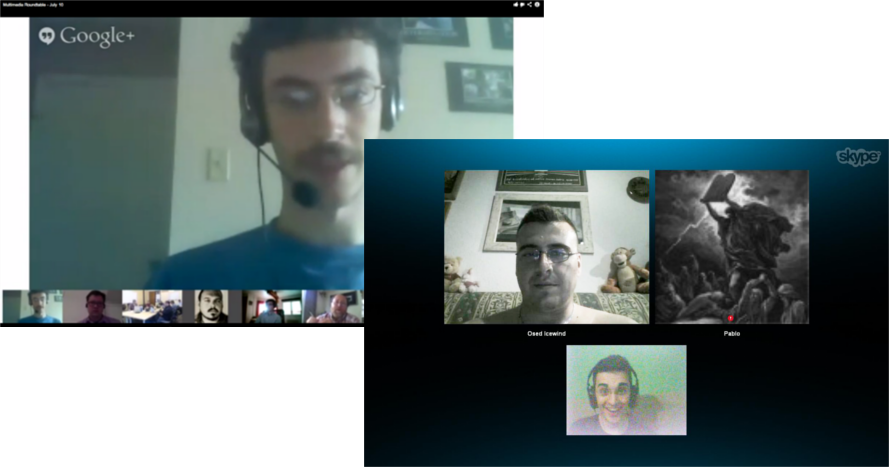
\includegraphics[keepaspectratio, scale=0.6]{Media/Captures/Soa/skype_hangouts.png}
  \caption{Hangouts and Skype}
  \label{fig:skype_hangouts}
\end{figure}
They focus on video, even hiding text communication to leave more room to the video. The Video Conference Gadget can be mixed with text above and below, leaving the video communication as an addition and not the main point. Both video communication tools shown (Google's Hangouts and Microsoft's Skype) require you to have a specific user account to use their services, while this gadget lets you join the video communication from within Wave, but also from an external link without giving any kind of personal information.

\subsubsection{Results}
To make this gadget it has been essential the use of a pre-existing service called appear.in that can be found in \verb|https://appear.in/|. They provide the whole video and audio communication, and also facilitate an easy way to use their service in an external website. It is a JavaScript component that can be put inside an iframe, and it will take care of almost everything. Figure \ref{fig:video_gadget} shows the final result of this integration.
\begin{figure}[H]
  \center
    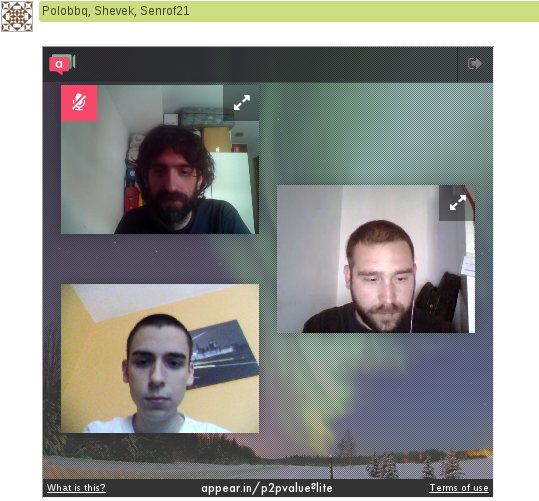
\includegraphics[keepaspectratio, scale=0.5]{Media/Captures/Extensions/VideoGadget.png}
  \caption{Video Conference Gadget}
  \label{fig:video_gadget}
\end{figure}
It was shown in Figure \ref{fig:gadget_classes} the basic structure of a gadget. The composite is represented by the VideoGadgetMainPanel, the Messages are the class VideoGadgetMessages, and the GinModule is realized by VideoGadgetGinModule. Outside from that, the structure is relatively simple.\\[.2cm]
As appar.in is a JavaScript service, multiple calls to native JavaScript have been made inside this gadget. To do that, you have to write the following pattern (Example for a private function returning a void type):
\begin{verbatim}
private native void function() /*-{
  Native JavaScript code goes here
}-*/;
\end{verbatim}
The service appear.in uses the name of the room as a unique identifier, so the gadget asks the user for a name before entering the room. The gadget also makes use of the \verb|?lite| feature, that simplifies the user interface, leaving more space for the images of the video. The camera is accessed through the browser, so no additional software has to be installed.\\[.2cm]
The Wave state in this gadget is really simple, the only thing stored in it is the name of the room to enter it directly if it has already been set.\\[.2cm]
The fact that this extension is completely dependant on an external closed-source service is a big limitation. The service could stop working at any time, technical improvements on video or audio communication can not be made, limitations like the maximum of 16 online users can not be avoided, the way to use it could change making it necessary to update the gadget...
